\begin{frame} \frametitle{\textit{Past work}: Theoretical microbubble dynamics in a viscoelastic medium at capillary breaching thresholds}
  \vspace*{\fill}
  \begin{minipage}{\textwidth}
    \begin{minipage}{0.3\textwidth}
      \visible<1->{
        \begin{figure}
          \centering
          \begin{tikzpicture}
            \node[anchor=south west,inner sep=0] (image) at (0,0) {
              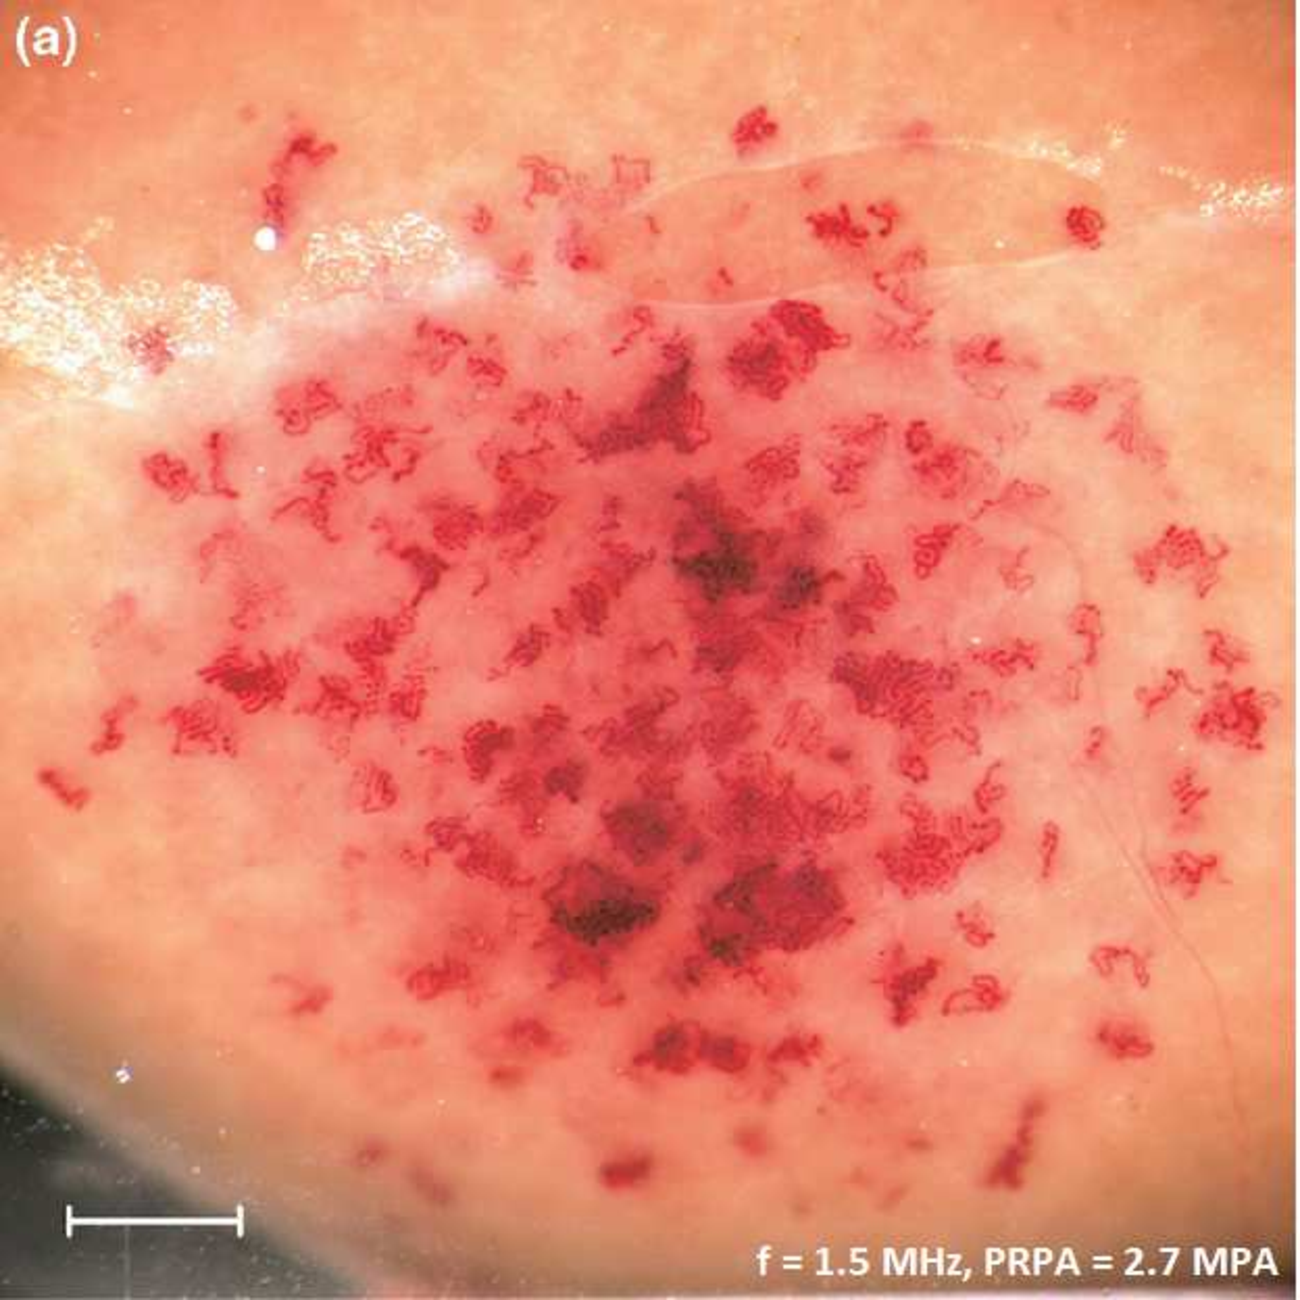
\includegraphics[width=0.8\textwidth]{./figs/Kidney_Bleed3}\hfill
            };%
            \begin{scope}[x={(image.south east)},y={(image.north west)}]%
              \node[font=\tiny,right] at (0.01,0.03) {\scalebox{0.4}{\textcolor{white}{\cite{Miller2008b}}}};%
            \end{scope}%  
          \end{tikzpicture}\hfill%
        \end{figure}
      }
    \end{minipage}
    \begin{minipage}{0.68\linewidth}
      
      {\tiny
        \visible<2->{
          \scalebox{0.9}{$
            \left(1-\frac{\dot{R}}{C}\right) R \ddot{R} + \frac{3}{2}\left(1-\frac{\dot{R}}{3 C}\right) \dot{R}^2 = \left(1+\frac{\dot{R}}{C}\right) \left[p_B- 1 -p_a -
              \frac{R}{C}\frac{dp_a}{dt}\right] +\frac{R}{C} \dot{p}_B,$\\}%
          \vspace*{2pt}
          \scalebox{0.9}{$p_B = \left(1+\frac{2}{We}\right)\frac{1}{R^{3\gamma}}-\frac{2}{WeR} + \tau_R,$\\}
        }
        \vspace*{0.5cm}
        \visible<3->{
          \begin{tabular}{l l c l}
            Parameter & Dimensional value & & Dimensionless number \\ \hline
            Viscosity & $\mu=0.015$ (Pa s) & $\mapsto$ & $Re=\rho u R_o / \mu = 2/3$ \\
            Elasticity & $G=10^5$ (Pa) & $\mapsto$ & $Ca= \rho u^2 / G = 1.0$ 	\\
            Surface tension & $S=0.056$ (N/m) & $\mapsto$ & $We=\rho u^2 R_o / S$ = 2 \\
            Sound speed & $c=1570$ (m/s) & $\mapsto$ & $C = c/u=157$ \\  
            % Relaxation time & $\lambda = 0.5$ ($\mu$ s) & $\mapsto$ &	$De=\lambda u / R_o =0$ \\
          \end{tabular}
        }
      }
    \end{minipage}
  \end{minipage}

  \vfill

  \begin{minipage}{\textwidth}
    % \includegraphics[width=0.6\textwidth]{../figs/bubble_figs/rt_nonlinear}\hfill
    \begin{figure}
      \visible<4->{
        \begin{tikzpicture}
          \node[anchor=south west,inner sep=0] (image) at (0,0) {%
            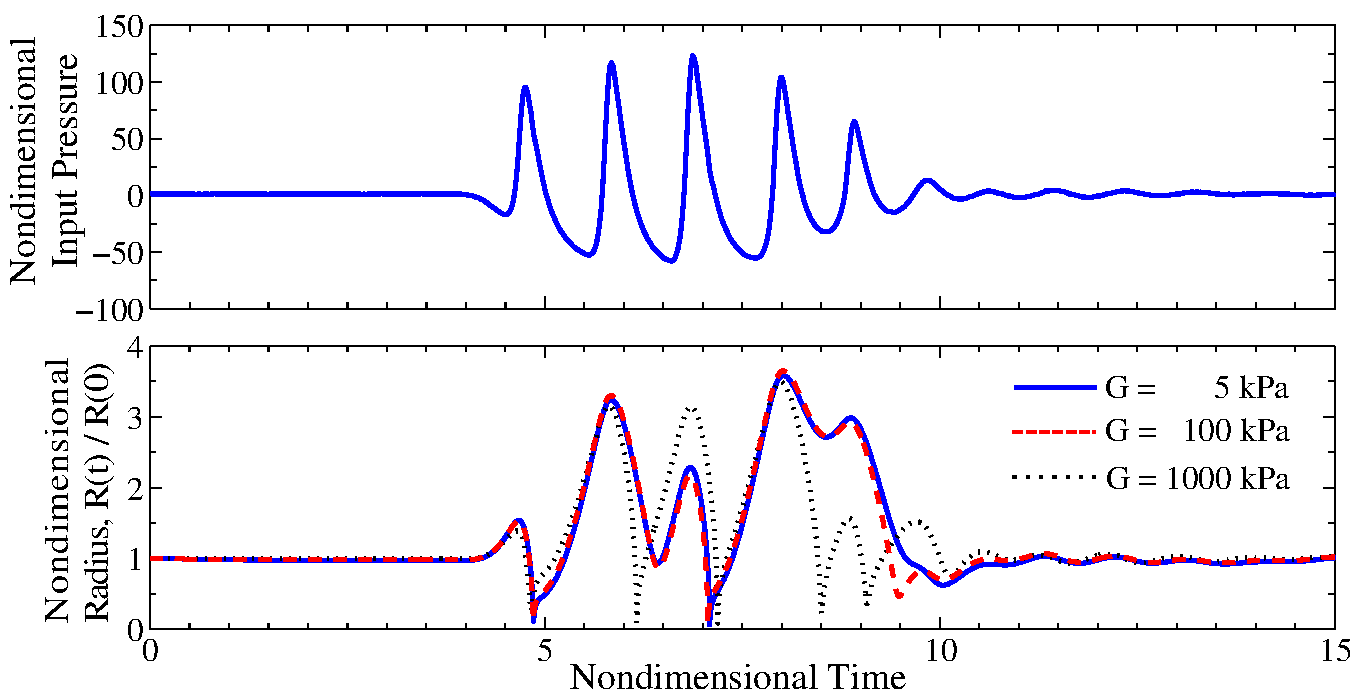
\includegraphics[width=0.57\textwidth]{../figs/bubble_figs/rt_nonlinear_flip_legend}\hfill%
          };%
          \begin{scope}[x={(image.south east)},y={(image.north west)}]%
            \node[font=\tiny,right] at (0.5,0.60) {\scalebox{0.7}{{7.5%
                  MHz Experimental Pressure Waveform}}};%
          \end{scope}%
        \end{tikzpicture}\hfill%
      }
      \visible<5->{
        \begin{tikzpicture}
          \node[anchor=south west,inner sep=0] (image) at (0,0) {%
            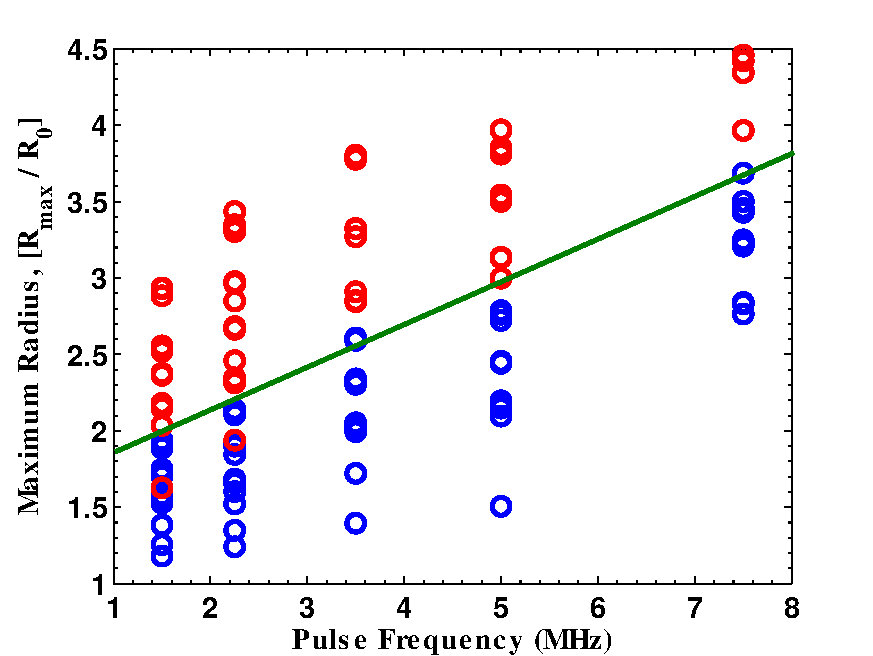
\includegraphics[width=0.4\textwidth]{../figs/bubble_figs/rstarmax_f2_1mpa}%
          };%
          \begin{scope}[x={(image.south east)},y={(image.north west)}]%
            \node[font=\tiny,right] at (0.57,0.15) {{$G=1000$ kPa}};%
          \end{scope}%
        \end{tikzpicture}
      }
    \end{figure}
  \end{minipage}
  \vfill
  \scalebox{0.7}{
    {\tiny Patterson, B., Miller, D. L., \& Johnsen, E. (2012). Theoretical microbubble dynamics in a viscoelastic medium at capillary breaching thresholds. JASA, 132(6), 3770.}
  }
\end{frame}

%%% Local Variables:
%%% mode: latex
%%% TeX-master: ../main
%%% End:
